\appendix
% \chapter{Annexes}

% TODO : C'est à écrire

% Liste des figures
\listoffigures
\glsaddallunused
\printglossaries

% Partie glossaire
%\printglossaries
%\glsaddallunused % < Pour ajouter les entrées non utilisées dans le texte


\chapter{Diagramme de gantt d'avancement du projet}

(Pour une lecture optimale, voir au verso)

\begin{sidewaysfigure}[h]
    \centering
    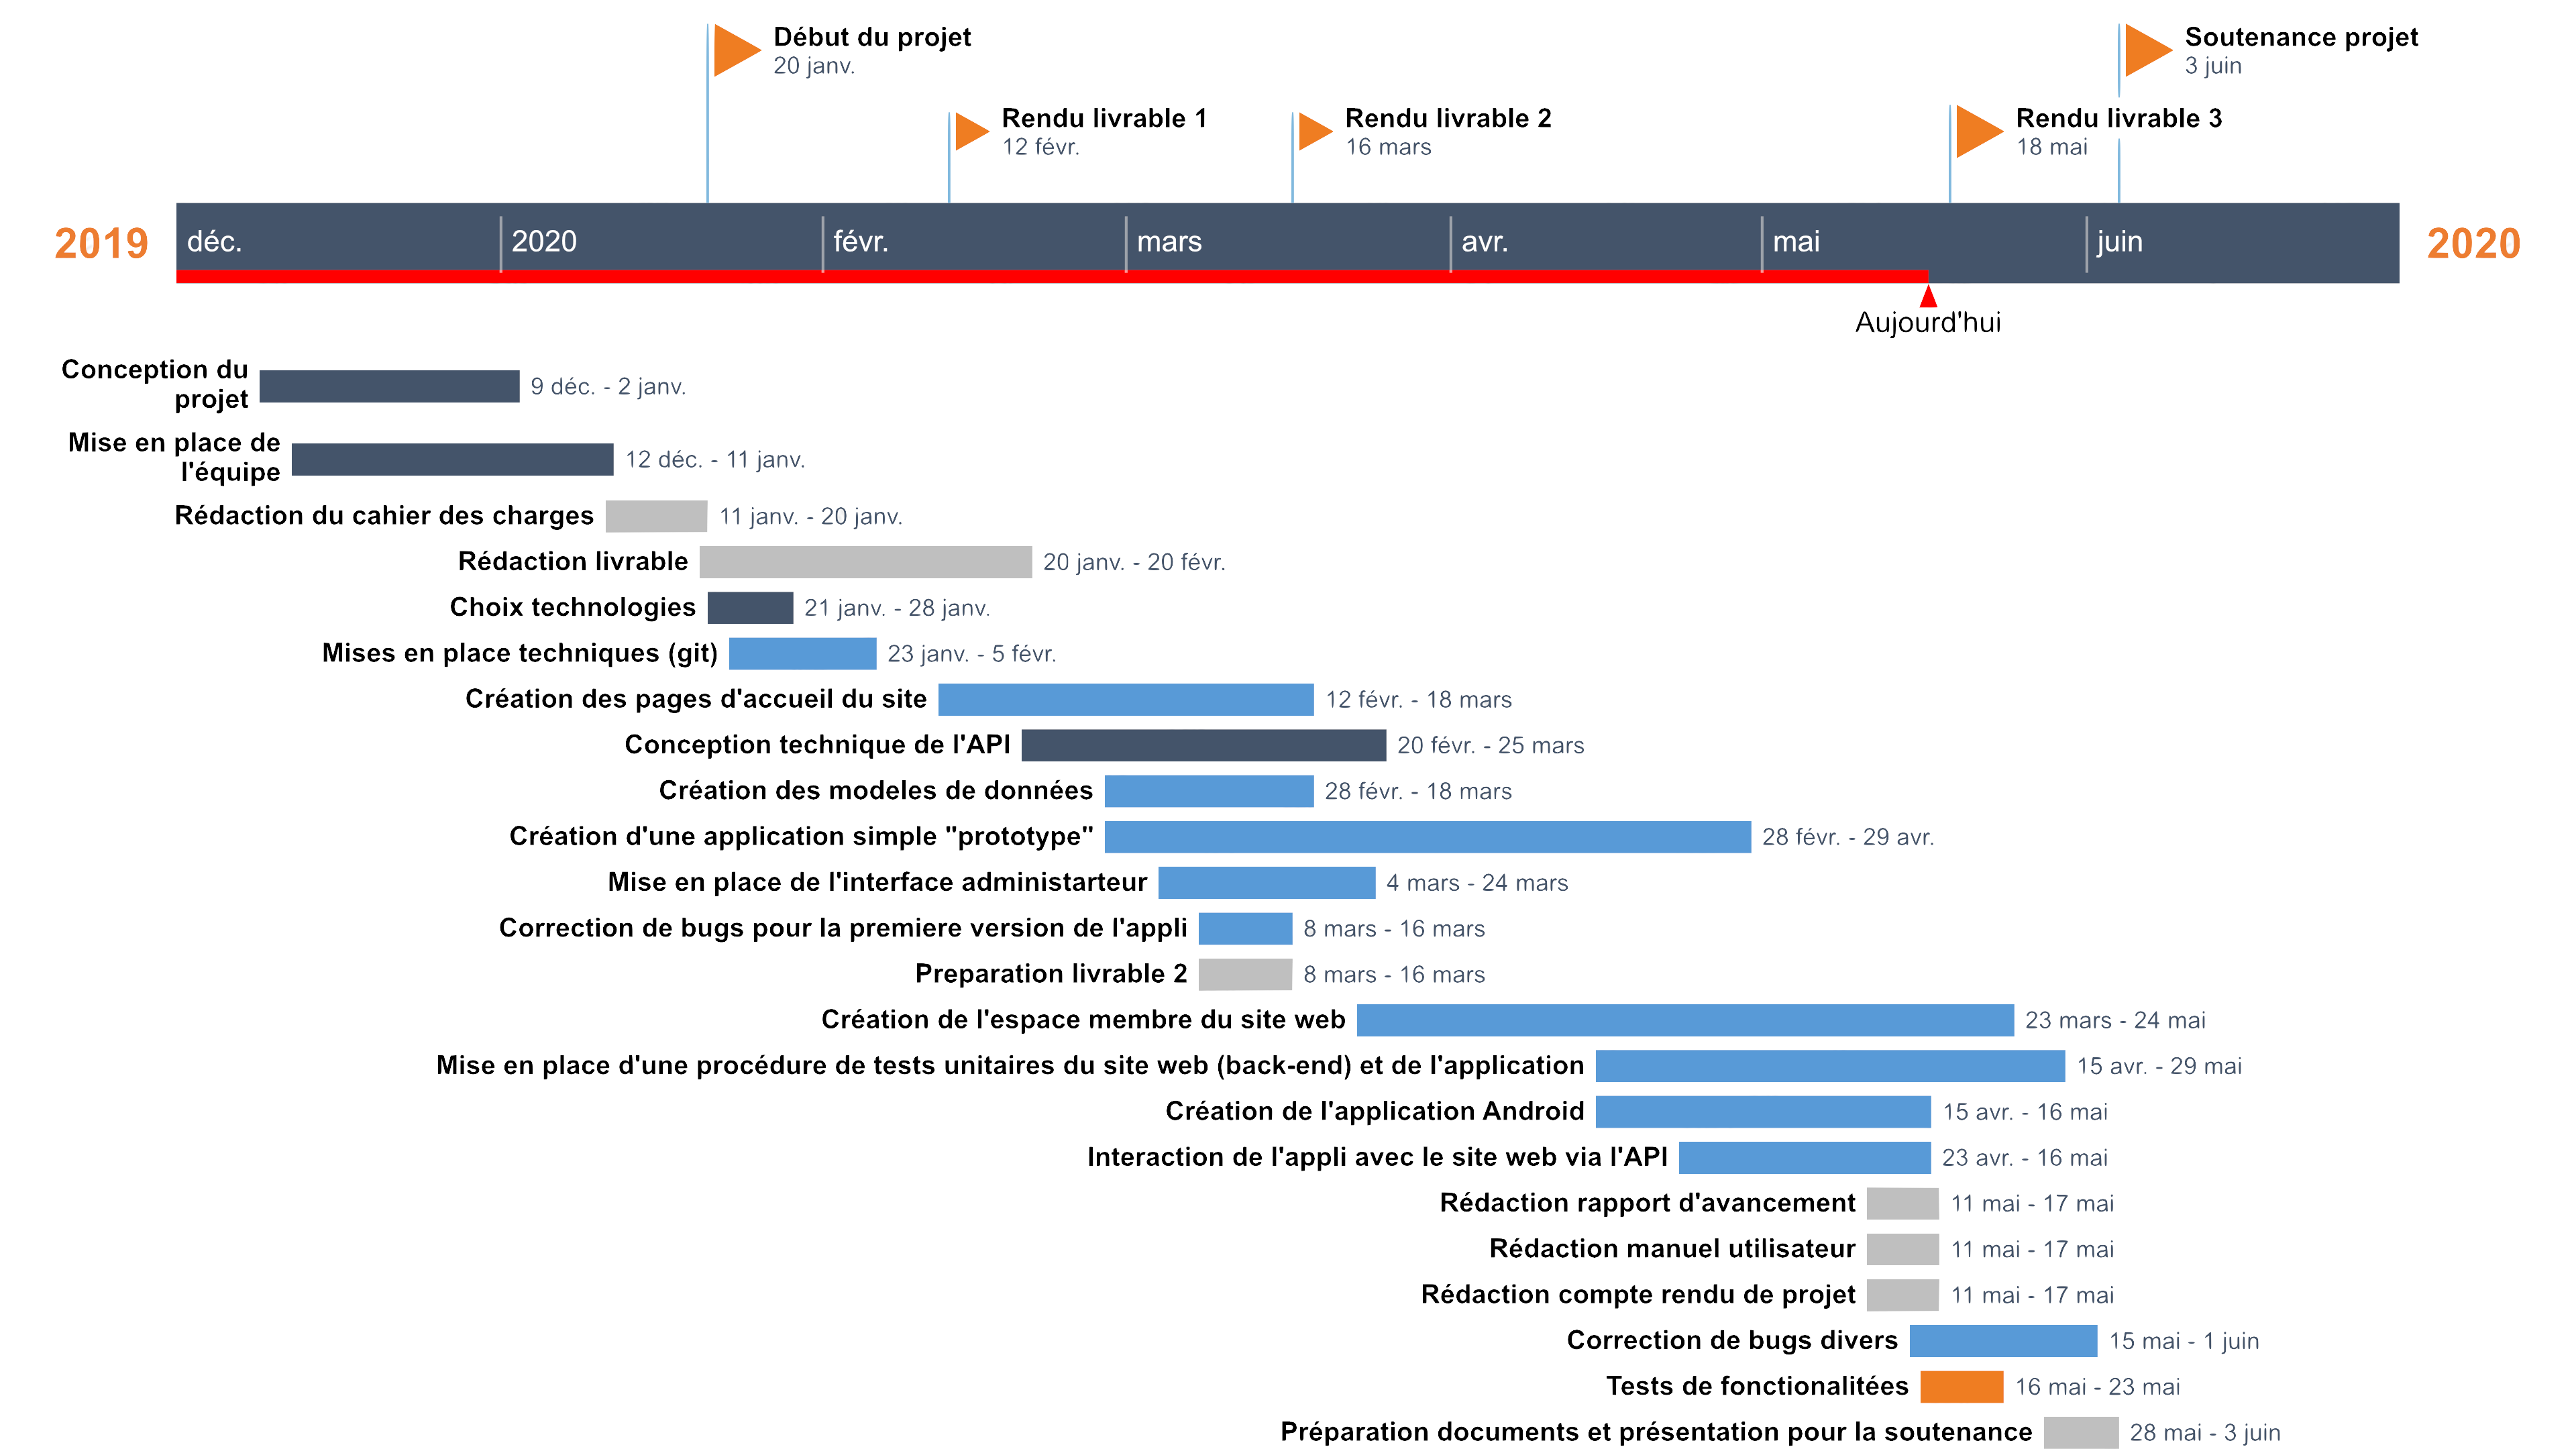
\includegraphics[keepaspectratio, width=\textwidth, height=\textheight]{ima/Planning-gantt}
    \caption{Planning effectif au 16 mai}
    \label{fig:91-Gantt}
\end{sidewaysfigure}


\chapter{Caddyfile pour le deployment du site web en production}

\begin{lstlisting}
(global) {
    # logs
    log {
        output file /var/log/caddy/access.log {
            roll_size 1gb
            roll_keep 5
            roll_keep_for 720h
        }
        format json
    }
    log
    file_server
}

(static_site) {
    import global
}

ghostrun.api-d.com {
    root * /var/www/ghostrun.api-d.com/GhostRun/GhostRunWeb/
    import static_site
    @notStatic {
        not path /static/* /media/*
    }
    reverse_proxy @notStatic localhost:8000
}
\end{lstlisting}